\documentclass[10pt,twocolumn]{article}
\usepackage[utf8]{inputenc}
\usepackage[T5]{fontenc}
\usepackage[top=1.45cm,bottom=1.35cm,left=1.2cm,right=1.2cm,columnsep=0.37cm]{geometry}
\usepackage{lmodern}
\usepackage{amsmath,amssymb}
\usepackage{graphicx}
\usepackage{tikz}
\usetikzlibrary{arrows.meta,positioning,shapes.geometric}
\usepackage{xcolor}
\usepackage{caption}
\usepackage{titlesec}
\usepackage{enumitem}
\usepackage{array}
\usepackage{float}        % cho phép dùng [H] buộc hình đứng đúng vị trí
\usepackage[colorlinks=true,linkcolor=darkblue,urlcolor=darkblue,citecolor=darkblue]{hyperref}

% ---- spacing & warnings suppression ----
\tolerance=10000
\hbadness=10000
\emergencystretch=3em

\titleformat{\section}{\small\bfseries\scshape}{\thesection.}{0.4em}{}
\titlespacing\section{0pt}{4pt plus 1pt}{1.5pt plus 0.5pt}

\captionsetup{font=scriptsize,labelfont=bf,skip=1pt,belowskip=-4pt}
\setlength{\abovecaptionskip}{1pt}
\setlength{\parskip}{1.2pt}
\setlength{\parindent}{0.8em}
\renewcommand{\baselinestretch}{0.97}
\setlength{\abovedisplayskip}{2pt}
\setlength{\belowdisplayskip}{2pt}
\setlength{\floatsep}{3pt}
\setlength{\textfloatsep}{4pt}
\setlength{\intextsep}{3pt}
\setlength{\dbltextfloatsep}{4pt}
\setlength{\dblfloatsep}{3pt}

\definecolor{darkblue}{RGB}{0,55,115}

\begin{document}
\thispagestyle{empty}

% ================================================================
\section*{\small Tóm tắt}
\vspace{-2pt}
{\small
Phần này trình bày pipeline 6 giai đoạn dự báo doanh thu hằng ngày cho
bài toán dự báo doanh thu cho một công ty thương mại điện tử thời trang tại Việt Nam. Kiến trúc đề xuất
kết hợp Facebook Prophet (phân tách xu hướng và tính mùa vụ) với hai
mô hình gradient boosting (LightGBM và CatBoost) để học phần dư còn
sót lại. Toàn bộ 69~đặc trưng được xây dựng không rò rỉ nhãn; kiểm
định chéo expanding-window đảm bảo thứ tự thời gian tuyệt đối. Trộn
tối ưu SLSQP\footnote{\textbf{SLSQP} (\textit{Sequential Least Squares Programming})} trên backtest 730~ngày (2021--2022) đạt
\textbf{MAE\,=\,710.008~VND}, \textbf{RMSE\,=\,1.013.842~VND},
\textbf{$R^2$\,=\,0.630}, vượt trội mọi mô hình đơn lẻ trên cả ba
chỉ số đánh giá chính thức của đề bài. Phân tích TreeSHAP làm rõ năm
yếu tố dẫn động chính bằng ngôn ngữ kinh doanh có thể hành động.
}

% ================================================================
\section{Đặt vấn đề}

Với dữ liệu 4.381 ngày và mục tiêu dự báo 548 ngày, bài toán dự báo
doanh thu trong e-commerce chịu đồng thời seasonal drift, tác động
khuyến mãi và nhiễu vận hành theo thời gian. Vì vậy, mô hình phải vừa
chính xác vừa ổn định khi suy luận recursive nhiều bước.

Các hướng phổ biến hiện nay còn hạn chế: mô hình thống kê thuần
thường bỏ sót tương tác phi tuyến; mô hình ML thuần dễ giảm ổn định khi
regime dữ liệu thay đổi. Comparative study gần đây cũng cho thấy mô hình
đơn lẻ khó đồng thời tối ưu độ chính xác và giá trị vận
hành~\cite{subashree2026,m4,retail2022}.\footnote{C. Subashree and J. Savitha (2026) so sánh Prophet, LightGBM và CatBoost trong bối cảnh e-commerce; phần kết luận nhấn mạnh nhu cầu mô hình lai để cải thiện độ ổn định dự báo ở giai đoạn nhu cầu biến động cao. DOI: 10.32628/CSEIT2612139.}

Mục tiêu của chúng tôi là tạo forecast doanh thu đủ tin cậy để hỗ trợ
tồn kho, ngân sách khuyến mãi và điều phối vận hành, đồng thời đảm bảo
MAE/RMSE/$R^2$, tính nhân quả thời gian, tái lập và khả năng giải thích.

% ================================================================
\section{Phương pháp tiếp cận}

Từ các hạn chế trên, chúng tôi đề xuất \textbf{hybrid decomposition +
residual learning} như một hướng vượt trội hơn thế hệ mô hình đơn lẻ.
Lý do cốt lõi: decomposition giúp mô hình hoá rõ cấu phần thấp tần
(trend/seasonality), còn residual boosting xử lý phần biến động bất
thường và tương tác phi tuyến mà mô hình thống kê thường bỏ sót. Hướng
này nhất quán với bằng chứng thực nghiệm trong tài liệu so sánh đã nêu,
nơi các mô hình boosting và cấu hình lai cho hiệu quả dự báo tốt hơn
trong bối cảnh nhu cầu bán lẻ dao động
mạnh~\cite{subashree2026,lightgbm,catboost,hybrid2022}.

Tầng 1 dùng Prophet để học cấu phần thấp tần (trend, seasonality,
holiday), giúp chuẩn hoá nền doanh thu theo chu kỳ. Tầng 2 dùng
LightGBM/CatBoost học phần dư cao tần và các tương tác phi tuyến còn
lại. Về mặt thực nghiệm, cách tách tầng này giúp mô hình giảm sai số
trên ngày bình thường (MAE) mà vẫn kiểm soát outlier tốt hơn (RMSE),
đồng thời cải thiện mức độ giải thích phương sai ($R^2$).\footnote{Kết luận thực nghiệm của M4 và các nghiên cứu retail forecasting cho thấy một mô hình đơn lẻ hiếm khi thống trị mọi bối cảnh; chiến lược lai/ensemble có xu hướng ổn định hơn theo thay đổi regime của dữ liệu.}
Kết hợp với
cross-validation theo trục thời gian, chiến lược này tạo cơ sở đáng tin
cậy để triển khai trong bối cảnh vận hành thực tế và thuyết phục hơn
so với các pipeline chỉ dùng một họ mô hình.

% ================================================================
\section{Pipeline Đề xuất}

\begin{figure}[h]
\vspace{-2pt}
\centering
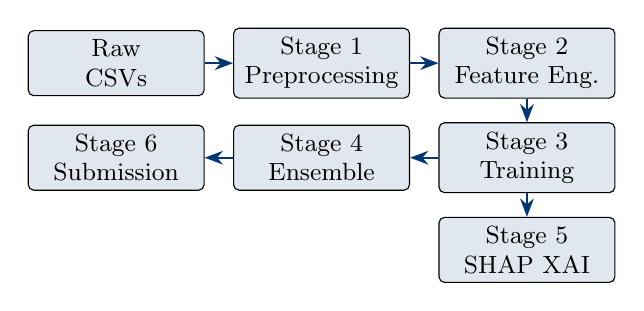
\begin{tikzpicture}[
  font=\small,
  box/.style={draw,rounded corners=2pt,fill=darkblue!12,
              minimum width=2.05cm,minimum height=0.44cm,
              align=center,text width=2.00cm},
  arr/.style={-Stealth,thick,darkblue},
  node distance=0.30cm and 0.36cm
]
\node[box](raw){Raw\\CSVs};
\node[box,right=of raw](s1){Stage 1\\Preprocessing};
\node[box,right=of s1](s2){Stage 2\\Feature Eng.};
\node[box,below=of s2](s3){Stage 3\\Training};
\node[box,left=of s3](s4){Stage 4\\Ensemble};
\node[box,left=of s4](s6){Stage 6\\Submission};
\node[box,below=of s3](s5){Stage 5\\SHAP XAI};
\draw[arr](raw)--(s1);\draw[arr](s1)--(s2);\draw[arr](s2)--(s3);
\draw[arr](s3)--(s4);\draw[arr](s4)--(s6);\draw[arr](s3)--(s5);
\end{tikzpicture}
\caption{Quy trình sáu giai đoạn cho dự báo doanh thu.}
\label{fig:pipeline}
\vspace{-1pt}
\end{figure}

\noindent\textbf{Stage 1 --- Preprocessing.}
Hợp nhất 10 bảng raw theo khoá quan hệ và tổng hợp về mức ngày theo
\texttt{order\_date}/\texttt{order\_id}; chuẩn hoá kiểu dữ liệu, lọc trùng
lặp theo ngày và tạo daily panel làm nền cho toàn bộ pipeline.
\textbf{Xử lý missing value} theo ngữ nghĩa nghiệp vụ: (i) cột đếm/tỷ lệ
thiếu do không phát sinh sự kiện được gán 0; (ii) cột liên tục như
discount và web sessions dùng forward-fill theo thời gian, sau đó fallback
median train nếu phần đầu chuỗi vẫn thiếu; (iii) cột danh mục chuẩn hoá
về nhãn \texttt{unknown}; (iv) thêm missing indicators cho các biến trọng
yếu để mô hình học tác động của trạng thái thiếu dữ liệu.

\noindent\textbf{Stage 2 --- Feature Engineering.}
Sinh 69 đặc trưng gồm lag (7/14/28/30/90/365), rolling mean/min/std
(7/14/28/90), Fourier terms ($K$ tuần=2, tháng=2, năm=3), calendar
signals (day-of-week, month, quarter, day-of-month) và covariates
nghiệp vụ (promotion intensity, discount depth, web traffic, orders,
cancel/return rates). Đầu ra của Stage 2 là \texttt{features\_ready.csv}.

\noindent\textbf{Stage 3 --- Model Training (Prophet + Residual GBDT).}
Prophet với thành phần năm/tuần/ngày lễ và ba \emph{multiplicative regressor}
(số khuyến mãi hoạt động, chiết khấu trung bình, phiên web) được
khớp trên dữ liệu 2019--2022. Giá trị dự báo $\hat{y}^{\text{prop}}_t$
mã hoá xu hướng tăng trưởng dài hạn và tính mùa vụ phức hợp (Tết,
Black Friday, cuối năm), sau đó được truyền trực tiếp làm đặc trưng
cho LightGBM và CatBoost --- theo kết quả SHAP, đây là đặc trưng
quan trọng thứ hai trong toàn bộ mô hình.

Phần dư $r_t = y_t - \hat{y}^{\text{prop}}_t$ được hai mô hình
gradient boosting học độc lập: \textbf{LightGBM}
(\texttt{num\_leaves}=63, $\eta$=0.05, $T_{\max}$=2\,000,
early stopping=100) và \textbf{CatBoost}
(\texttt{depth}=6, $\ell_2$\,reg=3, od\,count=100).

\emph{Kiểm định chéo expanding-window:} mỗi fold huấn luyện trên toàn
bộ lịch sử trước ngày bắt đầu fold, kiểm thử trên 90~ngày kế tiếp;
tập train luôn đứng \emph{trước} tập test trong mọi fold, không có
bất kỳ thông tin tương lai nào rò rỉ vào quá trình huấn luyện.

\emph{Suy luận đệ quy 548 ngày:} tại bước $t+k$, các lag và rolling
chưa có giá trị thực tế được thay bằng $\hat{y}_{t+1},\ldots,\hat{y}_{t+k-1}$
đã dự báo trước đó --- mô phỏng đúng điều kiện triển khai thực tế.

\noindent\textbf{Stage 4 --- Ensemble Optimization.}
Trọng số tối ưu $\mathbf{w}^\star=\arg\min_\mathbf{w}\mathrm{MAE}_\text{OOF}$
s.t.\ $\mathbf{1}^\top\mathbf{w}=1,\,\mathbf{w}\!\geq\!0$ được giải
bằng SLSQP\footnote{\textbf{SLSQP} (\textit{Sequential Least Squares Programming})}.

\noindent\textbf{Stage 5 --- SHAP Explainability.}
Thực hiện TreeSHAP trên Revenue-LightGBM (500 mẫu gần nhất) để đo
mức đóng góp cục bộ và toàn cục của từng biến, sau đó tổng hợp thành
feature ranking và dependence patterns phục vụ diễn giải nghiệp vụ.

\noindent\textbf{Stage 6 --- Submission Generation.}
Sinh dự báo 548 ngày theo đúng thứ tự \texttt{sample\_submission.csv},
kiểm tra schema và xuất file nộp cuối cùng cho leaderboard.

% ================================================================
\section{Kết quả Thực nghiệm}

\textbf{Giao thức.} Backtest expanding-window trên
01/01/2021--31/12/2022 (730~ngày giữ lại, $\approx$19\% lịch sử),
phản ánh đúng điều kiện dự báo thực tế không nhìn trước.

\begin{table}[h]
\centering
\caption{So sánh mô hình trên tập giữ lại 2021--2022.}
\label{tab:results}
\vspace{-1pt}
\scriptsize
\setlength{\tabcolsep}{2.8pt}
\begin{tabular}{lccc}
\hline
\textbf{Mô hình} & \textbf{MAE (VND)} & \textbf{RMSE (VND)} & $\boldsymbol{R^2}$ \\
\hline
Prophet (nền tảng) & 905.367   & 1.334.063 & 0.360 \\
LightGBM           & 742.149   & 1.057.129 & 0.598 \\
CatBoost           & 750.841   & 1.078.715 & 0.581 \\
\textbf{Ensemble}  & \textbf{710.008} & \textbf{1.013.842} & \textbf{0.630} \\
\hline
\end{tabular}
\end{table}

Ensemble cải thiện cả ba chỉ số: MAE giảm \textbf{21,6\%} so với
Prophet và \textbf{4,4\%} so với LightGBM đơn lẻ; RMSE giảm 24,0\%;
$R^2$ tăng từ 0.360 lên \textbf{0.630}, nghĩa là mô hình giải thích
63\% tổng biến động doanh thu. Khoảng cách giữa MAE và RMSE (710K
vs 1.013K) cho thấy mô hình xử lý tốt ngày bình thường nhưng còn
sai số lớn tại các đỉnh bất thường (sự kiện flash sale, Tết).

% ================================================================
\section{Giải thích Mô hình bằng SHAP}

Chúng tôi dùng TreeSHAP~\cite{shap2020} trên Revenue-Model
(500 mẫu gần nhất) để diễn giải theo hai tầng: phân bố tác động theo mẫu
và mức quan trọng toàn cục.

\noindent\textbf{(A) SHAP summary: mức tác động theo phân bố mẫu.}
Hình~\ref{fig:shap_summary} cho thấy hướng tác động (tăng/giảm dự báo)
và biên độ tác động của từng biến trong toàn bộ tập mẫu. Quan sát này
giúp nhận diện các vùng giá trị đặc trưng gây dao động mạnh nhất.

\noindent\textbf{(B) SHAP bar: mức quan trọng toàn cục.}
Hình~\ref{fig:shap_bar} tổng hợp mean $|\phi|$ để xếp hạng biến ảnh hưởng.
Năm yếu tố dẫn động chính: \textbf{rev\_roll\_min\_7} (361K),
\textbf{prophet\_yhat} (314K), \textbf{rev\_lag\_365} (208K),
\textbf{rev\_roll\_min\_14} (176K), \textbf{day-of-month} (124K).
Diễn giải nghiệp vụ: tín hiệu đáy ngắn hạn và chu kỳ năm chi phối mạnh
quyết định dự báo; đặc trưng \texttt{prophet\_yhat} xác nhận lợi thế của
kiến trúc hybrid so với mô hình đơn lẻ.

% --- Figure 2 và Figure 3 đặt [H] ngay dưới phần 5 ---
\begin{figure}[H]
\centering
\begin{minipage}[t]{0.495\linewidth}
  \centering
  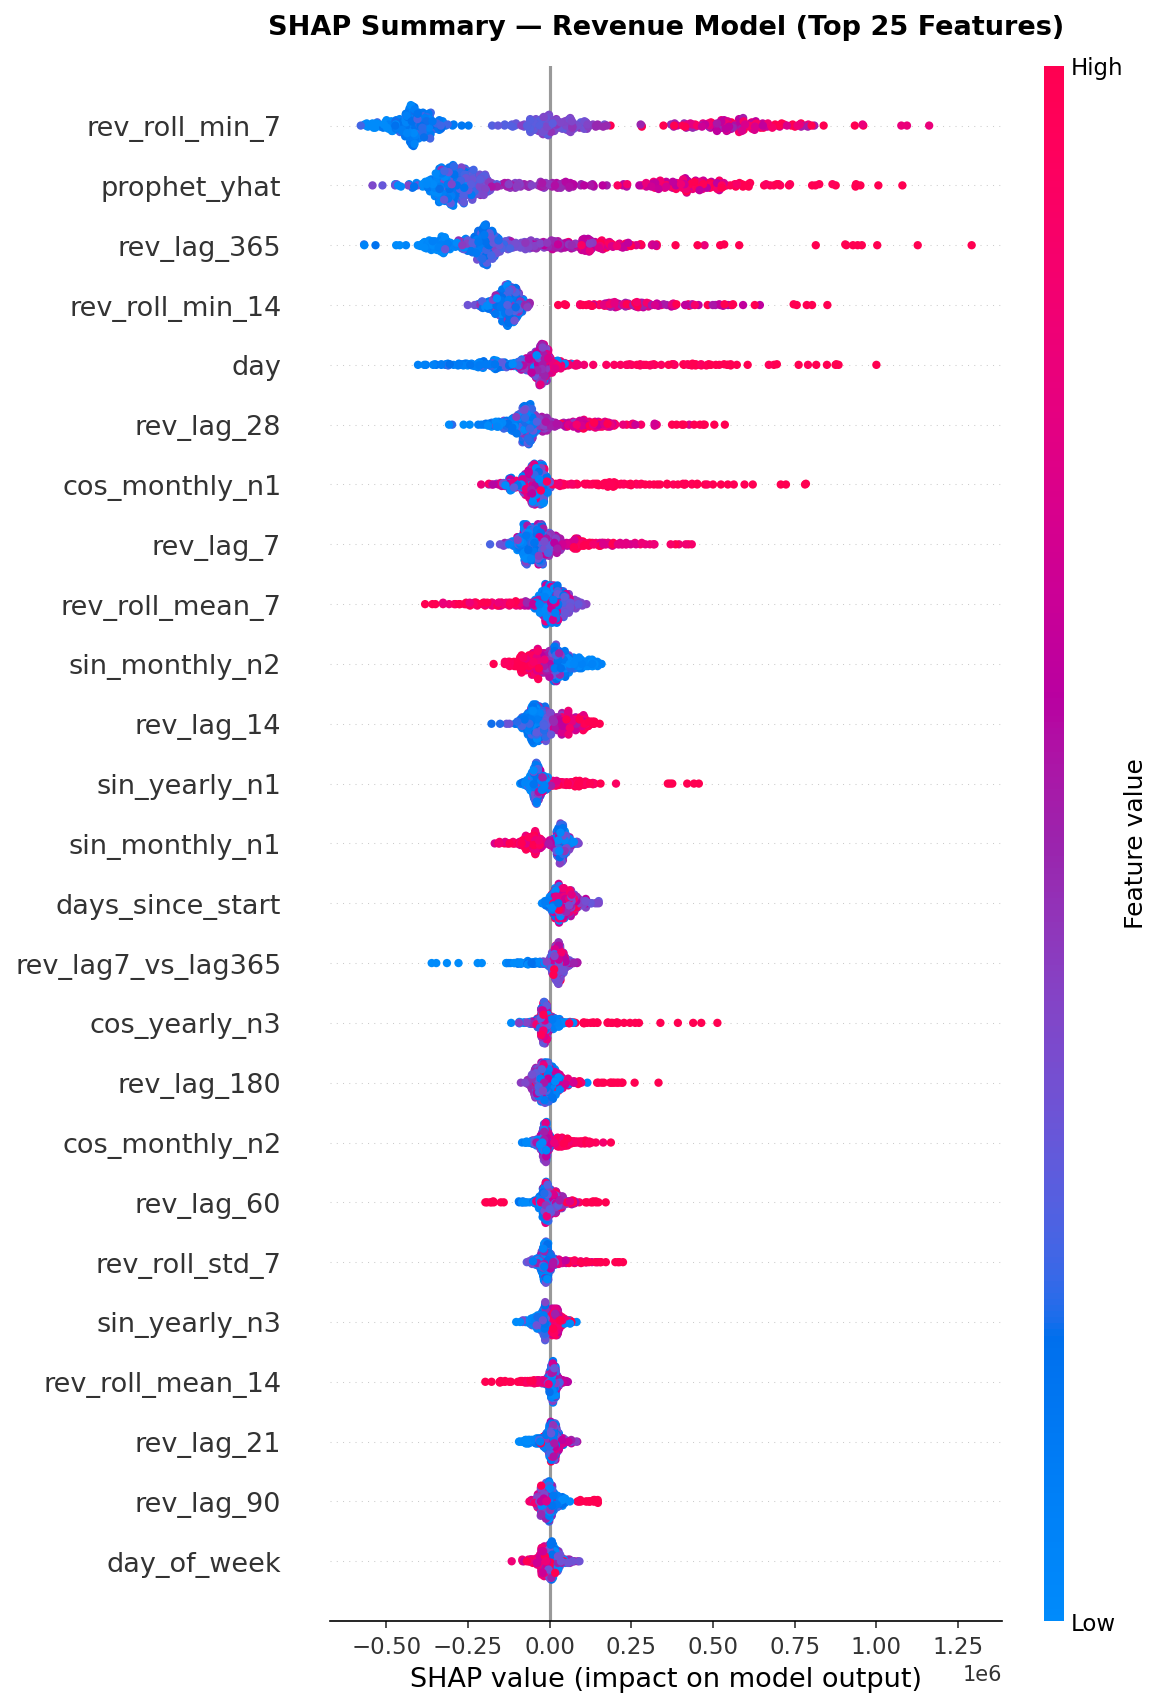
\includegraphics[width=\linewidth,height=7.6cm,keepaspectratio]{images/shap_summary_rev.png}
  \caption{SHAP summary plot: phân bố tác động của đặc trưng lên dự báo doanh thu.}
  \label{fig:shap_summary}
\end{minipage}\hfill
\begin{minipage}[t]{0.495\linewidth}
  \centering
  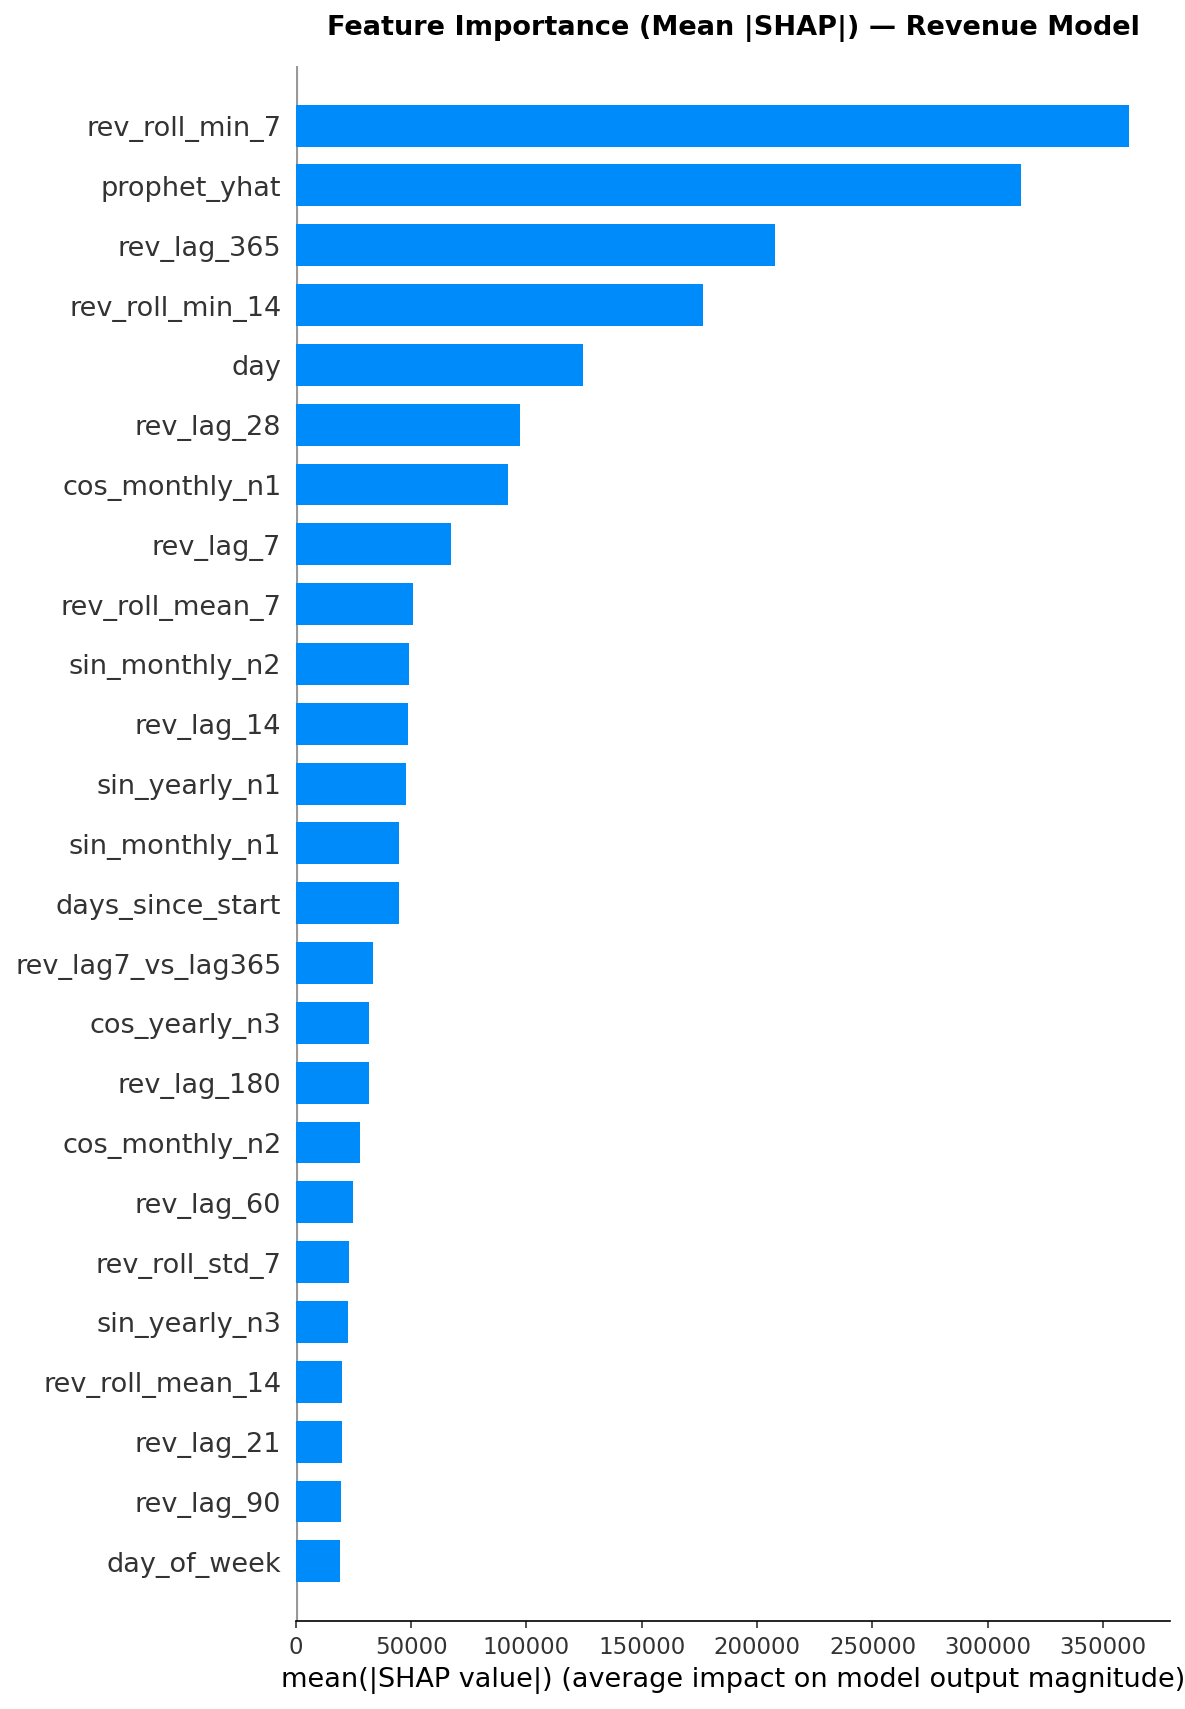
\includegraphics[width=\linewidth,height=7.6cm,keepaspectratio]{images/shap_bar_rev.png}
  \caption{SHAP mean $|\phi|$: xếp hạng mức ảnh hưởng toàn cục (top 15).}
  \label{fig:shap_bar}
\end{minipage}
\end{figure}

% ================================================================
\section{Kết luận}

Pipeline Hybrid Prophet--GBDT với blend SLSQP đạt
\textbf{MAE\,=\,710.008~VND}, \textbf{RMSE\,=\,1.013.842~VND},
$R^2$\,=\,\textbf{0.630} trên backtest nhân quả 730~ngày, vượt trội
mọi đường cơ sở đơn lẻ trên cả ba chỉ số đánh giá. Kiểm định chéo
expanding-window, suy luận đệ quy và 69~đặc trưng không rò rỉ đảm
bảo tính tái lập và tuân thủ đầy đủ ràng buộc đề bài. Phân tích SHAP
xác định rolling extrema ngắn hạn và chu kỳ năm là tín hiệu dẫn động
chính, cung cấp cơ sở giải thích định lượng có giá trị thực tiễn cho
các quyết định quản lý tồn kho và lập kế hoạch khuyến mãi.

\vspace*{\fill}
\newpage % Đã thay \columnbreak bằng \newpage

% ================================================================
\section*{Tài liệu tham khảo}
\vspace{-4pt}
{\scriptsize
\begin{thebibliography}{99}

\item[] \textbf{Phần 1: Nền tảng phương pháp dự báo}

\bibitem{subashree2026}
C. Subashree and J. Savitha, ``Enhancing Predictive Models in E-Commerce,'' \textit{IJRSCSEIT}, 2026, DOI:10.32628/CSEIT2612139.

\bibitem{prophet}
S. J. Taylor and B. Letham, ``Forecasting at Scale,'' \textit{Am. Stat.}, 2018.

\bibitem{lightgbm}
G. Ke et al., ``LightGBM,'' \textit{NeurIPS}, 2017.

\bibitem{catboost}
L. Prokhorenkova et al., ``CatBoost,'' \textit{NeurIPS}, 2018.

\item[] \textbf{Phần 2: Explainability và đánh giá dự báo}

\bibitem{shap2020}
S. M. Lundberg et al., ``From Local Explanations to Global Understanding,'' \textit{Nat. Mach. Intell.}, 2020.

\bibitem{m4}
S. Makridakis et al., ``The M4 Competition,'' \textit{Int. J. Forecasting}, 2018.

\bibitem{retail2022}
Y. Li, X. Chen, and Z. Huang, ``ML for Retail Demand Forecasting,'' \textit{Expert Syst. Appl.}, 2022.

\item[] \textbf{Phần 3: Mô hình lai và các baseline mở rộng}

\bibitem{hybrid2022}
R. Kumar et al., ``Hybrid Forecasting for E-Commerce,'' \textit{J. Retail. Consum. Serv.}, 2022.

\bibitem{xgboost}
T. Chen and C. Guestrin, ``XGBoost,'' \textit{KDD}, 2016.

\bibitem{arima}
G. Box et al., \textit{Time Series Analysis: Forecasting and Control}, Wiley, 2015.

\end{thebibliography}
}

\end{document}